%%%%%%%%%%%%%%%%%%%%%%%%%%%%%%%%%%%%%%
%%%%%%%%%%%%%%%%%%%%%%%%%%%%%%%%%%%%%%
% Do not edit the TeX file your work
% will be overwritten.  Edit the RnW
% file instead.
%%%%%%%%%%%%%%%%%%%%%%%%%%%%%%%%%%%%%%
%%%%%%%%%%%%%%%%%%%%%%%%%%%%%%%%%%%%%%




We consider a modification to the expected number of posterior clusters defined in 
equation~\ref{eq:expected_num_clusters}. We wish to measure the number of clusters with at least $t$ observations rather than the total number of distinct clusters. Hence we may also consider the posterior quantity 
\begin{align}
g_t(\etathetaopt) &:=
\Expect_{q(z \vert \etazopt(\eta_\theta))} \left[ \#\{\text{clusters with at least $t$ datapoints}\} \right]  \\
&=
\Expect_{q(z \vert \etazopt(\eta_\theta))} \left[
    \sum_{k=1}^K \mathbb{I}\left\{\left(\sum_{n=1}^N \mathbb{I}\{z_n \ne k\} \right) > t \right\}\right].
    \label{eq:expected_num_clusters_thresh}
\end{align}
Note that $t = 0$ reduces to the original target posterior defined in the equation~\ref{eq:expected_num_clusters}. 

This equation defines an \textit{in-sample} quantity. We also consider a posterior predictive quantity, that is, the number of clusters we expect see in a new dataset. This is an expectation over the variational distribution of the sticks $\nu$, defined as 
\begin{align}
g_{t, pred}(\etathetaopt) &:=
\Expect_{q(\nu \vert \eta_\nu^{*}(\eta_\theta))} \left[\#\{\text{clusters with at least $t$ datapoints}\} \right]  \\
&=
\Expect_{q(\nu \vert \eta_\nu^{*}(\eta_\theta))} \left[\sum_{k=1}^K \left(1 - \sum_{i = 1}^t {t\choose i}
\pi_k^{i} (1 - \pi_k)^{t - i}\right)\right].
    \label{eq:expected_num_clusters_pred_thresh}
\end{align}
where $\pi_k$ are the cluster probabilities induced by the the sticks $\nu$. 

Figure~\ref{fig:param_sens_plot_thresh_0} shows both the in-sample and predictive expected number of \textit{distinct} clusters (i.e. $t = 0$). 


\begin{knitrout}
\definecolor{shadecolor}{rgb}{0.969, 0.969, 0.969}\color{fgcolor}\begin{figure}[!h]

{\centering 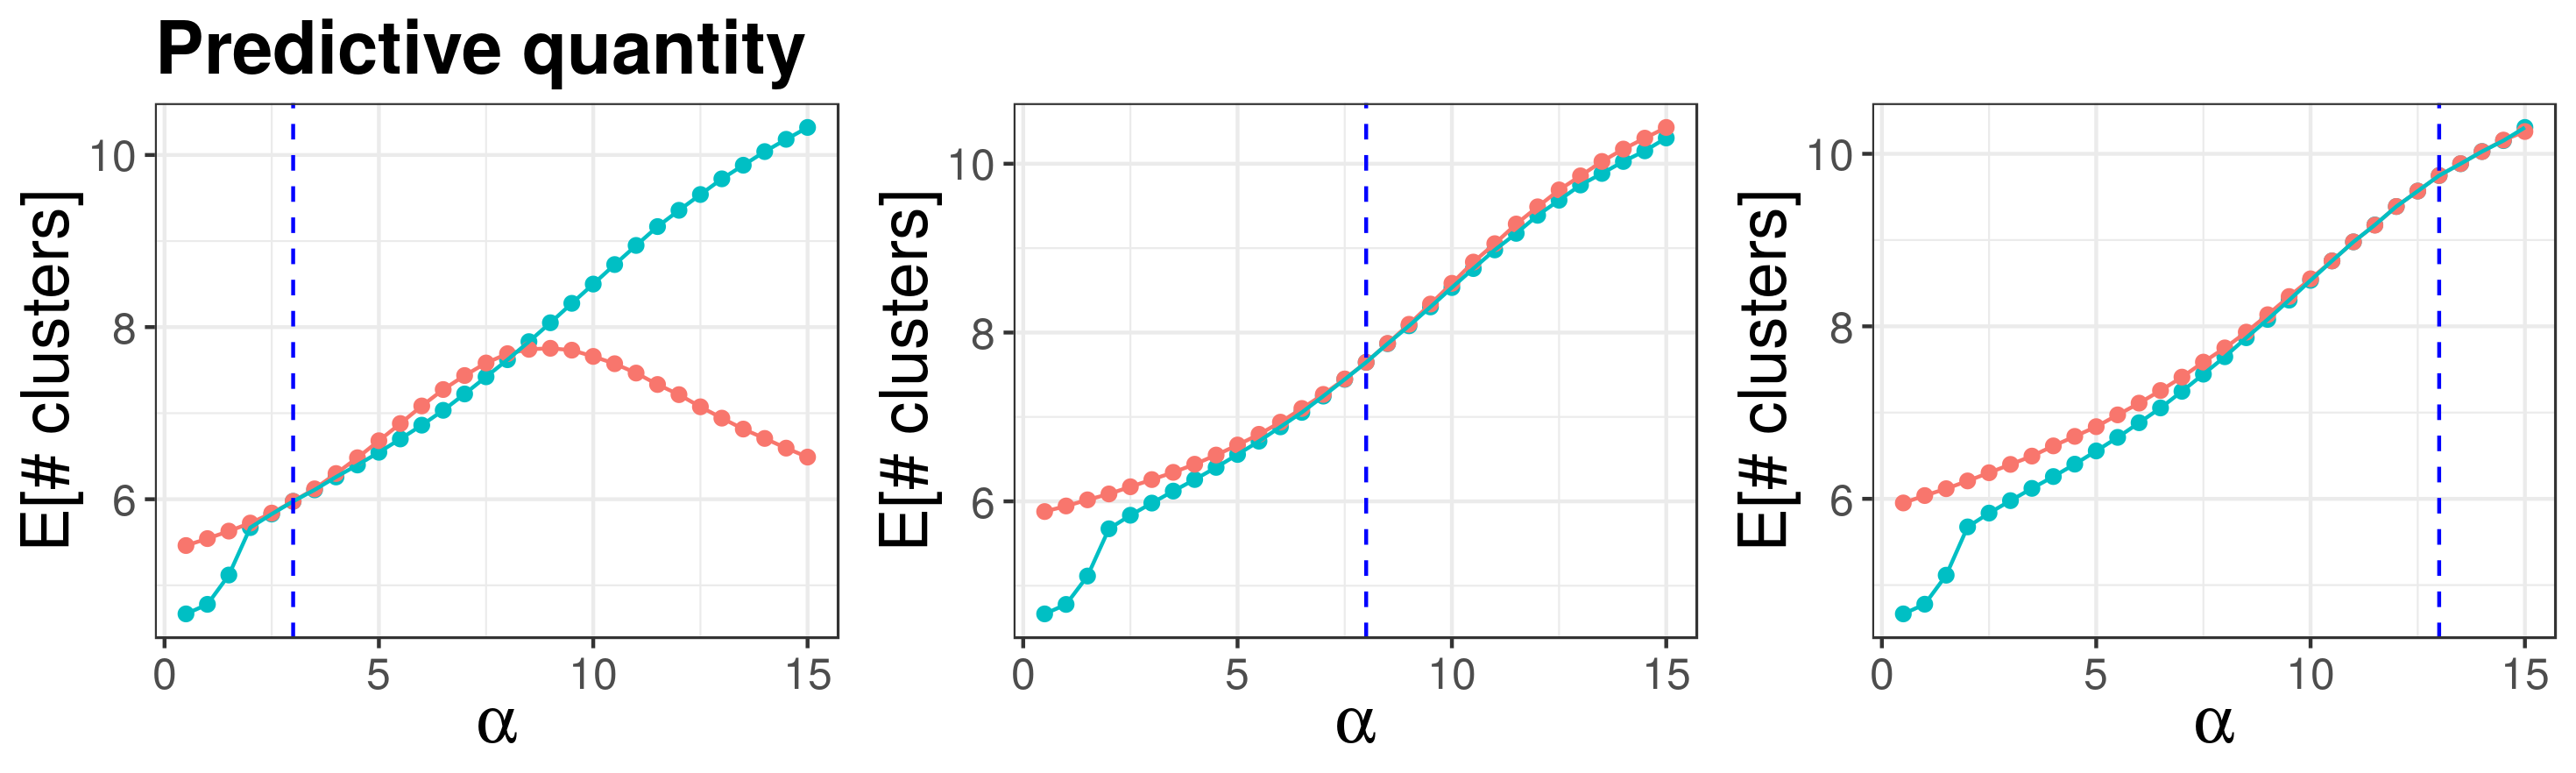
\includegraphics[width=0.98\linewidth,height=0.294\linewidth]{figure/param_sens_plot_thresh_0-1} 
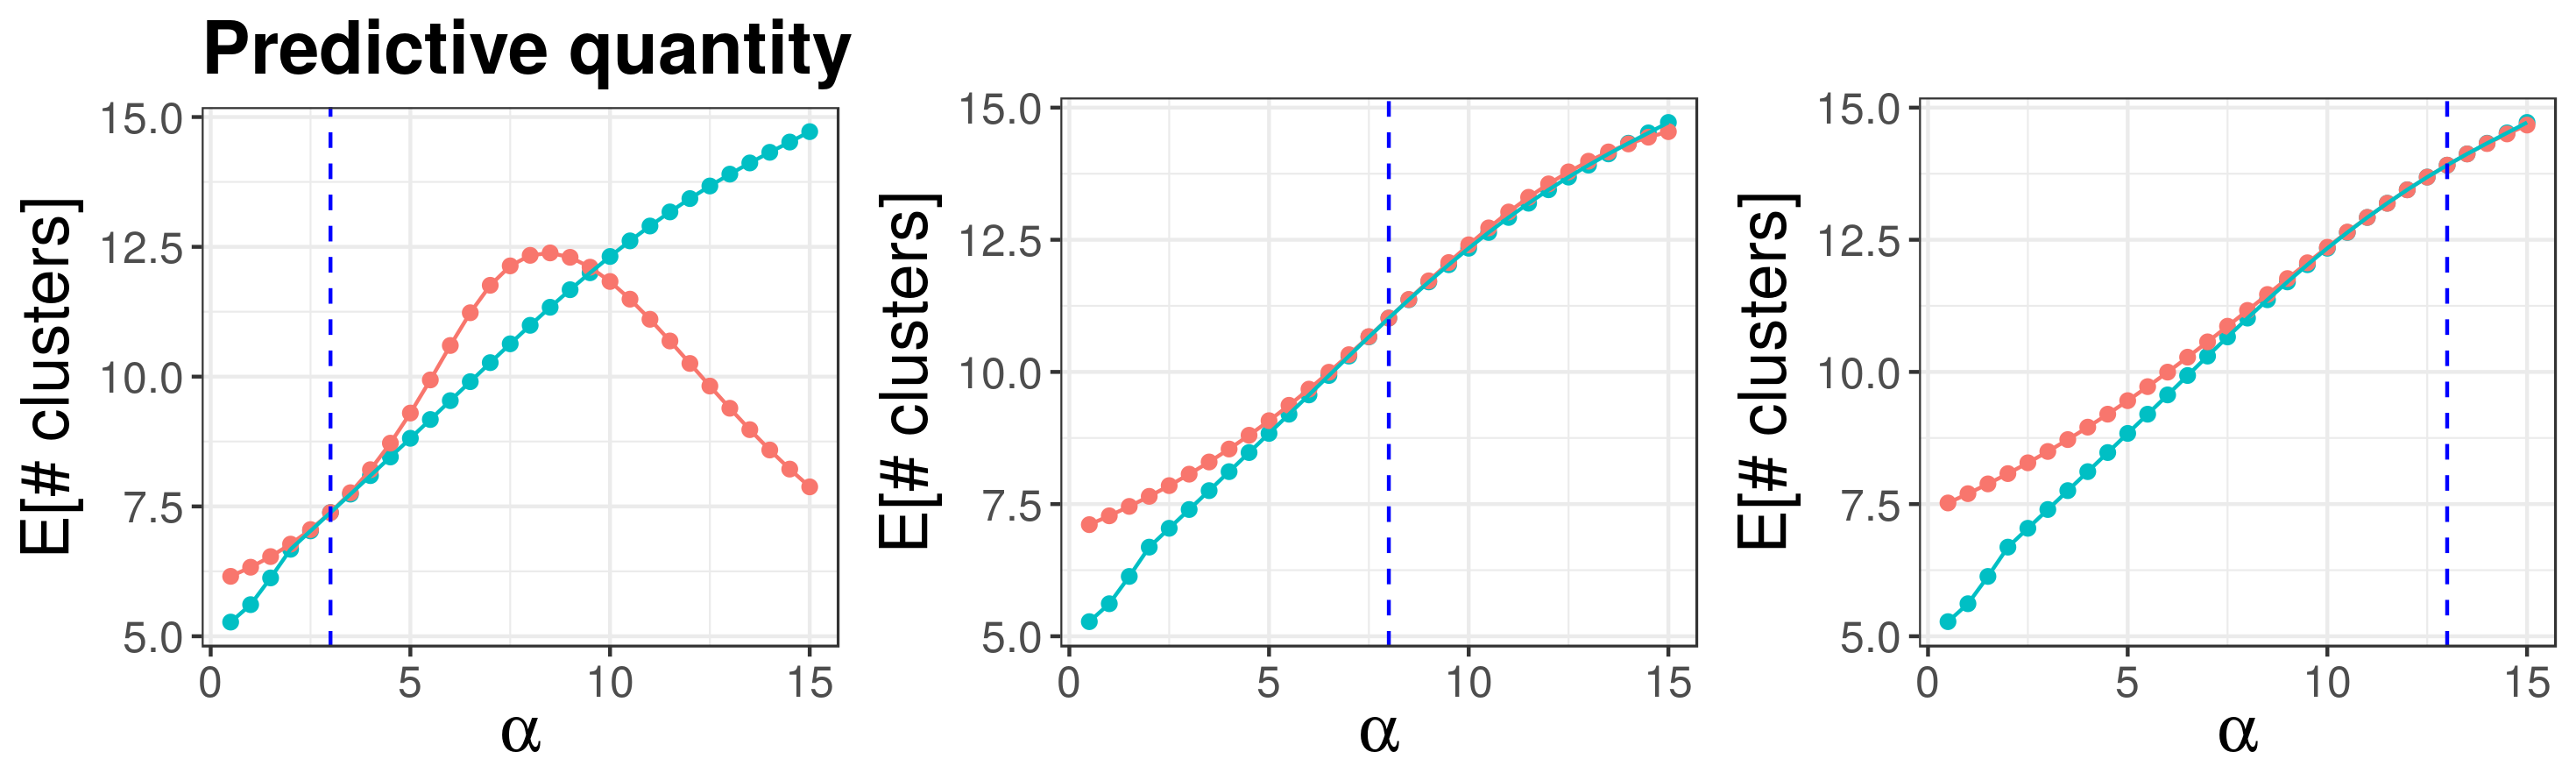
\includegraphics[width=0.98\linewidth,height=0.294\linewidth]{figure/param_sens_plot_thresh_0-2} 

}

\caption[The in-sample expected number of distinct clusters (Top), and the predictive expected number of distinct clusters (Bottom)]{The in-sample expected number of distinct clusters (Top), and the predictive expected number of distinct clusters (Bottom). Comparison of these values computed by re-optimizing versus the linear approximation.  The blue vertical line indicates the location of $\alpha_0$.}\label{fig:param_sens_plot_thresh_0}
\end{figure}


\end{knitrout}

Next, figure~\ref{fig:param_sens_plot_thresh_3} shows both the in-sample and predicted expected number of clusters with at least three observations ($t = 3$). 

The linear approximation does equally well in both cases, and works best when we set $\alpha_0 = 13$, and approximate from having more clusters to fewer clusters. 


\begin{knitrout}
\definecolor{shadecolor}{rgb}{0.969, 0.969, 0.969}\color{fgcolor}\begin{figure}[!h]

{\centering 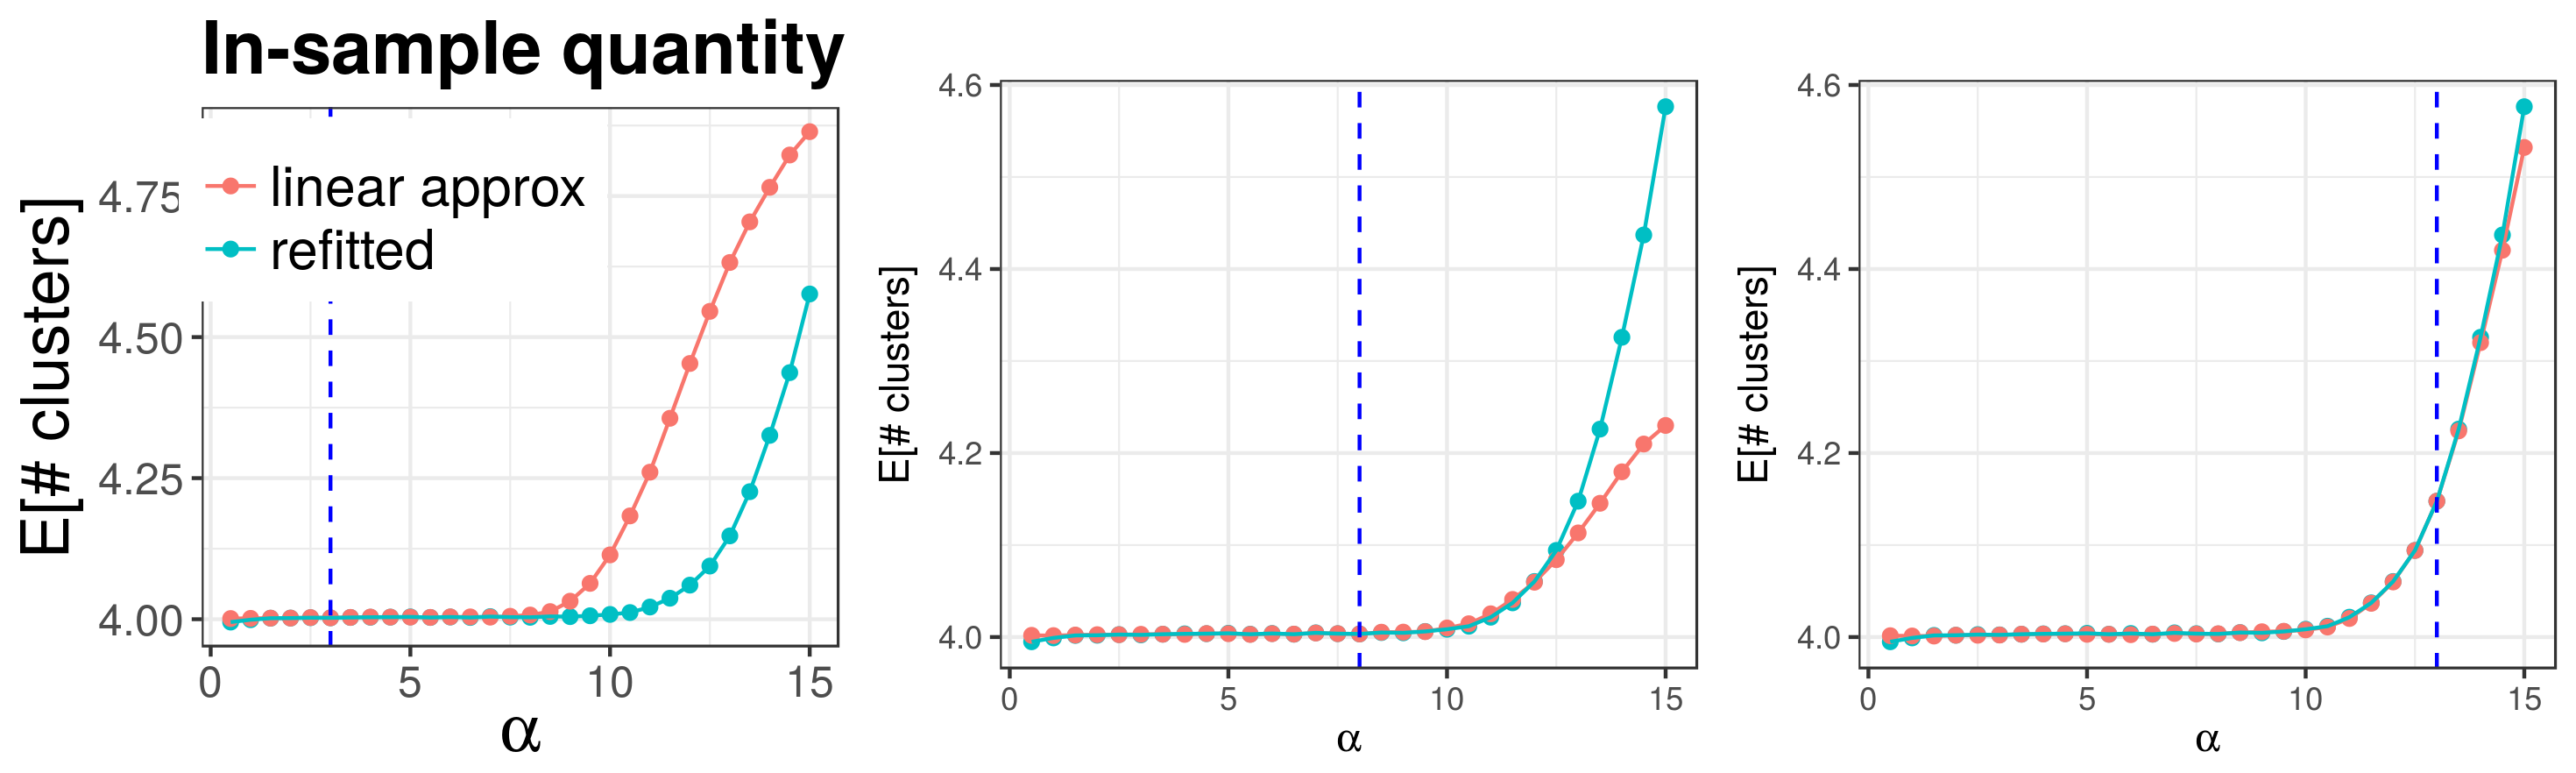
\includegraphics[width=0.98\linewidth,height=0.294\linewidth]{figure/param_sens_plot_thresh_3-1} 
\includegraphics[width=0.98\linewidth,height=0.294\linewidth]{figure/param_sens_plot_thresh_3-2} 

}

\caption[The in-sample expected number of distinct clusters with at least three observations (Top), and the corresponding predictive quantity (Bottom)]{The in-sample expected number of distinct clusters with at least three observations (Top), and the corresponding predictive quantity (Bottom). Comparison of these values computed by re-optimizing versus the linear approximation.  The blue vertical line indicates the location of $\alpha_0$.}\label{fig:param_sens_plot_thresh_3}
\end{figure}


\end{knitrout}
